\subsection{Auswirkung der verschiedenen Rechenverfahren für die Position}
Um die Qualität der Berechnung auf verschiedenen Distanzen zu ermitteln, wurde der Datensatz Forests for Real Time 3D Face Analysis \cite{database_Face_Ori} verwendet, da für jedes Gesicht die Position und Orientierung bekannt ist.
Die durchschnittliche Distanz zwischen Kamera und Kopf beträgt ca $70cm$ bei einer Kopfbreite von 78 Pixel. Um die verschiedenen Distanzen zwischen Probanden und Kamera zu simulieren, wurden die Bilder mit dem angegebene Skalierungsfaktor (X-Achse) linear verkleinert.\\
Da verschiedene Verfahren zur Bestimmung der Position und Orientierung zur Verfügung stehen, sollen diese miteinander verglichen werden. Zur Bestimmung wurde nur das RGB-Bild verwendet und nicht zusätzlich die Tiefenaufnahme, da diese in der Anwendung auch nicht vorhanden ist.
\subsubsection{Position}
Zur Bestimmung der Position gibt es zwei Verfahren, die direkte mittels Brennweite und Skalierung oder Überführungsmatrix von 3D zu 2D Landmarks arbeiten.\\
Die Funktionen PoseCamera und PoseWorld verwenden die einfache Bestimmung mittels Skalierung und CorrectPoseCamera und CorrectPoseWorld die Überführung von 3D und 2D Landmarks, daher überlagern sich die Linien in \autoref{img_Verfahren_Pos}, da die jeweiligen Verfahren nach dem selben Prinzip rechnen.\\
Der schnelle Abfall der Genauigkeit bei der Skalierung $0,25$ ist an der selben Stelle an der auch die Detektionsrate stark absinkt, siehe \autoref{OpenFace_skal}. Somit kann das Verfahren bis zu seiner Grenze eingesetzt werden und erst, wenn die Detektion schwierig wird steigt auch der Fehler.
\begin{figure}
	\centering
	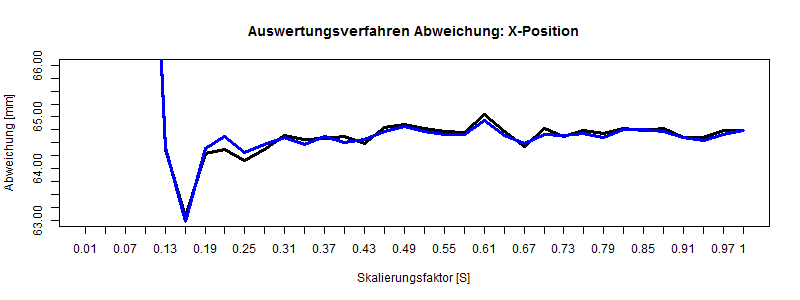
\includegraphics[width=\linewidth]{img_Skalierung/Verfahren_TX}
	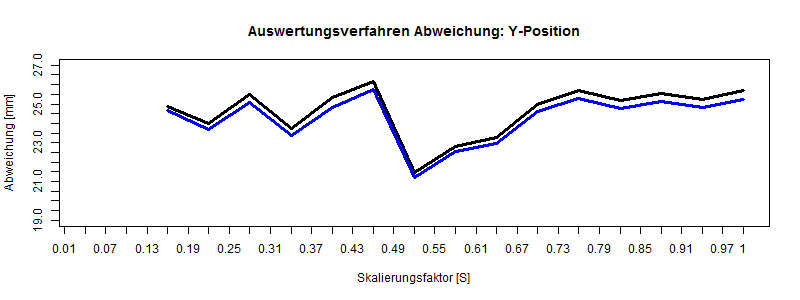
\includegraphics[width=\linewidth]{img_Skalierung/Verfahren_TY}
	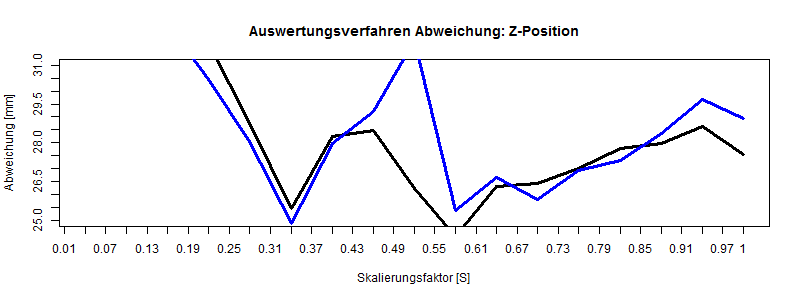
\includegraphics[width=\linewidth]{img_Skalierung/Verfahren_TZ}
	\caption{Dargestellt ist der Median der Abweichung in Millimeter der Positionsbestimmung auf Bilder die mit Lanczos skaliert wurden.\\
	PoseWorld (schwarz), PoseCamera (rot, verdeckt von PW), CorrectPoseCamera (grün, verdeckt von CPW) und CorrectPoseWorld (blau)\\
	Oben: X-Position, Mitte: Y-Position, Unten: Z-Position}
	\label{img_Verfahren_Pos}
\end{figure}
\subsubsection{Orientierung}
Bei der Rotation zeigen sich nun Unterschiede zwischen den einzelnen Verfahren, da bei PoseWorld und CorrectPoseWorld auch die Position im Kamerabild berücksichtigt wird.\\
Aus \autoref{img_Verfahren_Rot} ist zu entnehmen, dass die zusätzliche Korrektur das Ergebnis weiter verbessert wird, wenn die Pixelorientierungen mit beachtet werden.
\begin{figure}
	\centering
	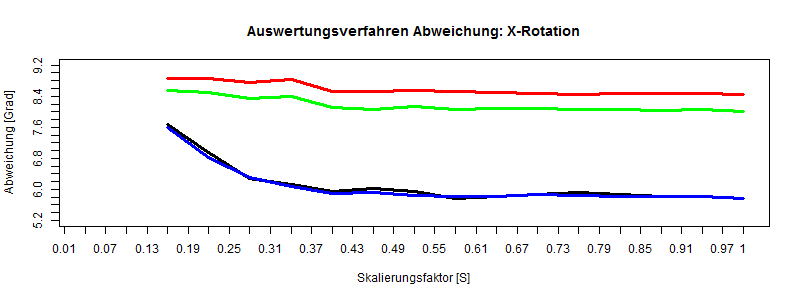
\includegraphics[width=\linewidth]{img_Skalierung/Verfahren_RX}
	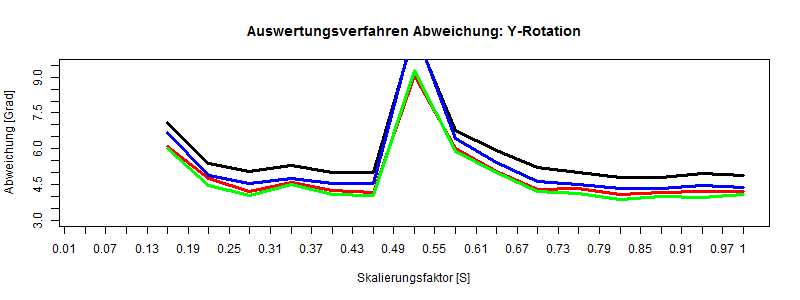
\includegraphics[width=\linewidth]{img_Skalierung/Verfahren_RY}
	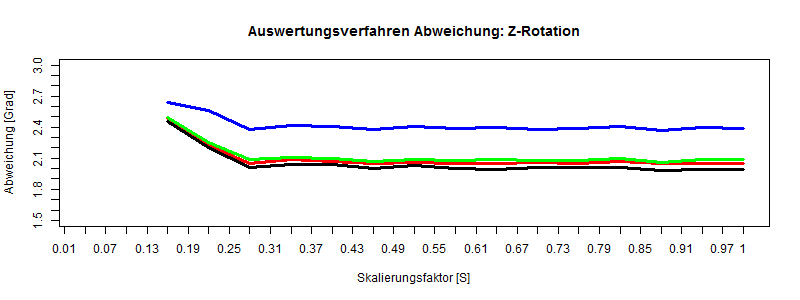
\includegraphics[width=\linewidth]{img_Skalierung/Verfahren_RZ}
	\caption{Dargestellt ist der Median der Abweichung in Grad der Positionsbestimmung auf Bilder die mit Lanczos skaliert wurden.\\
		PoseWorld (schwarz), PoseCamera (rot), CorrectPoseCamera (grün) und CorrectPoseWorld (blau)\\
		Oben: X-Rotation, Mitte: Y-Rotation, Unten: Z-Rotation}
	\label{img_Verfahren_Rot}
\end{figure}
\subsubsection{Ergebnis}
Es zeigt sich, dass CorrectPoseWorld, also die komplexe Bestimmung der Position mittels 2D/3D Landmarks und zusätzlicher Korrektur der Winkel die besten Ergebnisse liefert im Test.\\
Im Test ist die Überführung von 3D zu 2D Landmarks am besten (CorrectPoseCamera und CorrectPoseWorld) kann sich allerdings auch ändern wenn die Kamera Parameter besser abgeschätzt sind, da ohne eine Tiefenaufnahme die korrekte Überführung nur geschätzt werden kann und sich Fehler fortpflanzen können.